\noindent

\includegraphics[height=1.25cm]{images/pictograms/replication}

\includegraphics[height=1.25cm]{images/pictograms/benchmark}

\includegraphics[height=1.25cm]{images/pictograms/under_construction}

\includegraphics[height=1.25cm]{images/pictograms/FDM}
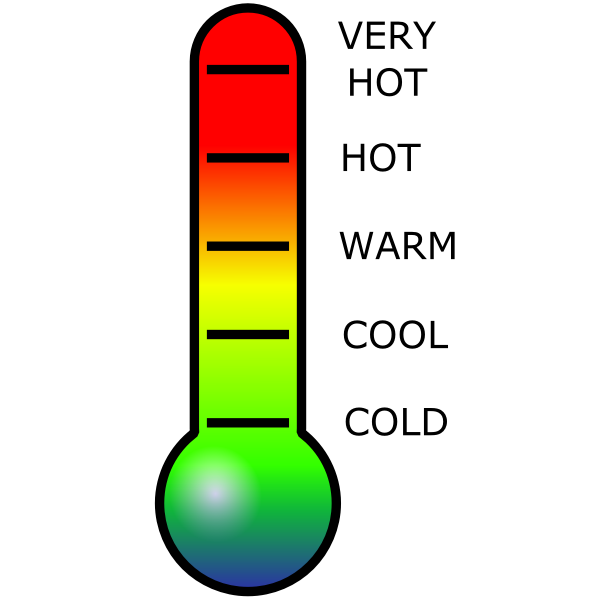
\includegraphics[height=1.25cm]{images/pictograms/temperature}

\includegraphics[height=1.25cm]{images/pictograms/paraview}
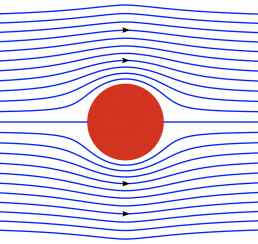
\includegraphics[height=1.25cm]{images/pictograms/streamfunction}


%%%%%%%%%%%%%%%%%%%%%%%%%%%%%%%%%%%%%%%%%%%%%%%%%%%%%%%%%%%%%%%%%%%%%%%%%%%%%%%%%%%%%%%%%%%%%%%%%%%

\begin{flushright} {\tiny {\color{gray} python\_codes/fieldstone\_155/text.tex}} \end{flushright}

%\lstinputlisting[language=bash,basicstyle=\small]{python_codes/template_keywords.key}

\par\noindent\rule{\textwidth}{0.4pt}

\begin{center}
\inpython
{\small Code: \url{https://github.com/cedrict/fieldstone/tree/master/python_codes/fieldstone_155}}
\end{center}

\par\noindent\rule{\textwidth}{0.4pt}

%%%%%%%%%%%%%%%%%%%%%%%%%%%%%%%%%%%%%%%%%%%%%%%%%%%%%%%%%%%%%%%%%%%%%%%%%%%%%%%%%%%%%%%%%%%%%%%%%%%


This \stone computes the 2-D thermal convection of a fluid 
of infinite Prandtl number in a unit square closed cell as described in \textcite{blbc89}.
The mass, momentum, energy equations are solved by means of the Finite Difference method
applied to a vorticity-stream function formulation.

The temperature is fixed to zero on the top and to $\Delta T=1$ at the bottom, 
with reflecting symmetry at the sidewalls (i.e. $\partial_x T=0$) 
and there are no internal heat sources. 
Free-slip conditions are implemented on all boundaries. 
Models are run for $\Ranb=10^{3,4,5,6}$.

The initial temperature field is given by 
\begin{equation}
T(x,y)=(1-y) - 0.01\cos(\pi x) \sin(\pi y)
\end{equation}
The perturbation in the initial temperature fields leads to 
a perturbation of the density field and sets the fluid in motion. 
Depending on the Rayleigh number, the system ultimately reaches a 
steady state after some time (the higher the Rayleigh number, the larger this time). 
Note that at $t=0$, we have
\[
\frac{\partial T}{\partial x} = 0.01 \pi \sin(\pi x)
\]
which we need in the context of the stream function.

The Nusselt number (i.e. the mean surface temperature gradient over 
mean bottom temperature)
is computed as follows \cite{blbc89}:
\begin{equation}
\Nunb = L_y \frac{\int_0^{L_x} \frac{\partial T}{\partial y}(y=L_y) \; dx  }{\int_0^{L_x} T(y=0) \; dx}
\label{eqNu}
\end{equation}
Note that in our case the denominator is equal to 1 since $L_x=1$ 
and the temperature at the bottom is prescribed to be 1.

If no convection is taking place (i.e. $\Ranb$ is too low) then 
only diffusion is taking place 
and the steady state temperature field is then $T(y)=1-y$, 
so that $\partial_y T=-1$ and we find that the Nusselt number is simply 1.

The equations to be solved are as follows:
\begin{eqnarray}
\vec\nabla^2 \omega &=& -\Ranb \frac{\partial T}{\partial x} \\
\vec\nabla^2 \Psi   &=&  -\omega \\
\frac{\partial T}{\partial t} + \vec\upnu \cdot \vec\nabla T - \vec\nabla^2 T   &=& 0
\qquad \text{with} \qquad 
\vec\upnu=(\partial \Psi/\partial y,-\partial \Psi / \partial x)
\end{eqnarray}

%%%%%%%%%%%%%%%%%%%%%%%%%%%%
\section*{Discretisation}

The vorticity and stream function PDEs are Poisson equations and we use a 2nd order 
stencil (see Section~\ref{MMM-XXX}). Boundary conditions are specified here after.


When it comes to the energy equation, we have to solve a PDE of the type:
\[
\frac{\partial T}{\partial t} = {\cal F}(\vec \upnu,\vec\nabla T,\Delta T)
\]
with ${\cal F}(\vec \upnu,\vec\nabla T,\Delta T)=(-\vec\upnu\cdot\vec\nabla T + \vec\nabla\cdot k\vec\nabla T)$.
The (explicit) forward Euler method is: 
\[
\frac{T^{n}-T^{n-1}}{\delta t} = {\cal F}^{n-1}(\vec \upnu,\vec\nabla T,\Delta T)
\]
but we know this results in an unstable scheme.
The (implicit) backward Euler method is: 
\[
\frac{T^{n}-T^{n-1}}{\delta t} = {\cal F}^{n}(\vec \upnu,\vec\nabla T,\Delta T)
\]
which is better, 
and the (implicit) Crank-Nicolson algorithm is: 
\[
\frac{T^{n}-T^{n-1}}{\delta t} = 
\frac{1}{2}
\left[
{\cal F}^{n}(\vec \upnu,\vec\nabla T,\Delta T)
+
{\cal F}^{n-1}(\vec \upnu,\vec\nabla T,\Delta T)
\right]
\]
where the superscript $n$ indicates the time step.
The Crank-Nicolson is obviously based on the trapezoidal rule, with second-order convergence in time.

In the fully implicit case the energy equation is discretised as follows:
\[
\frac{T_{i,j}^n-T_{i,j}^{n-1}}{\delta t} =
- u^n_{i,j} \frac{T^n_{i+1,j}-T^n_{i-1,j}}{2h_x}
- v^n_{i,j} \frac{T^n_{i,j+1}-T^n_{i,j-1}}{2h_y}
+ \frac{T^n_{i+1,j}-2T^n_{i,j}+T^n_{i-1,j}}{h_x^2}
+ \frac{T^n_{i,j+1}-2T^n_{i,j}+T^n_{i,j-1}}{h_y^2}
\]
or,
\begin{footnotesize}
\[
\left(1 +\frac{2 \delta t}{h_x^2} +\frac{2 \delta t}{h_y^2} \right)  T^n_{i,j}
-\left(\frac{u^n_{i,j} \delta t}{2h_x} +\frac{\delta t}{h_x^2} \right) T^n_{i-1,j}
-\left(\frac{v^n_{i,j} \delta t}{2h_y} +\frac{\delta t}{h_y^2} \right) T^n_{i,j-1}+
\left(\frac{u^n_{i,j} \delta t}{2h_x} -\frac{\delta t}{h_x^2} \right)  T^n_{i+1,j}+
\left(\frac{v^n_{i,j} \delta t}{2h_y} -\frac{\delta t}{h_y^2} \right)  T^n_{i,j+1}
=
T_{i,j}^{n-1}
\]
\end{footnotesize}
In the Crank-Nicolson case the energy equation is discretised as follows:
\begin{eqnarray}
\frac{T_{{\color{teal} i,j}}^n-T_{i,j}^{n-1}}{\delta t} 
&=& 
- u^n_{{\color{teal} i,j}} \frac{T^n_{i+1,j}-T^n_{i-1,j}}{4h_x}
- v^n_{{\color{teal} i,j}} \frac{T^n_{i,j+1}-T^n_{i,j-1}}{4h_y}
+ \frac{T^n_{i+1,j}-2T^n_{{\color{teal} i,j}}+T^n_{i-1,j}}{2h_x^2}
+ \frac{T^n_{i,j+1}-2T^n_{{\color{teal} i,j}}+T^n_{i,j-1}}{2h_y^2} \nn\\
&&
- u^{n-1}_{i,j} \frac{T^{n-1}_{i+1,j}-T^{n-1}_{i-1,j}}{4h_x}
- v^{n-1}_{i,j} \frac{T^{n-1}_{i,j+1}-T^{n-1}_{i,j-1}}{4h_y}
+ \frac{T^{n-1}_{i+1,j}-2T^{n-1}_{i,j}+T^{n-1}_{i-1,j}}{2h_x^2}
+ \frac{T^{n-1}_{i,j+1}-2T^{n-1}_{i,j}+T^{n-1}_{i,j-1}}{2h_y^2} \nn
\end{eqnarray}


\begin{eqnarray}
\frac{T_{{\color{teal} i,j}}^n-T_{i,j}^{n-1}}{\delta t} 
&+& 
  u^n_{{\color{teal} i,j}} \frac{T^n_{i+1,j}-T^n_{i-1,j}}{4h_x}
+ v^n_{{\color{teal} i,j}} \frac{T^n_{i,j+1}-T^n_{i,j-1}}{4h_y}
- \frac{T^n_{i+1,j}-2T^n_{i,j}+T^n_{i-1,j}}{2h_x^2}
- \frac{T^n_{i,j+1}-2T^n_{i,j}+T^n_{i,j-1}}{2h_y^2} \nn\\
&=&
- u^{n-1}_{{\color{teal} i,j}} \frac{T^{n-1}_{i+1,j}-T^{n-1}_{i-1,j}}{4h_x}
- v^{n-1}_{{\color{teal} i,j}} \frac{T^{n-1}_{i,j+1}-T^{n-1}_{i,j-1}}{4h_y}
+ \frac{T^{n-1}_{i+1,j}-2T^{n-1}_{i,j}+T^{n-1}_{i-1,j}}{2h_x^2}
+ \frac{T^{n-1}_{i,j+1}-2T^{n-1}_{i,j}+T^{n-1}_{i,j-1}}{2h_y^2} \nn
\end{eqnarray}

{\small
\begin{eqnarray}
T_{i,j}^n
&+& 
  u^n_{i,j} \frac{T^n_{i+1,j}-T^n_{i-1,j}}{4h_x} \delta t
+ v^n_{i,j} \frac{T^n_{i,j+1}-T^n_{i,j-1}}{4h_y}\delta t
- \frac{T^n_{i+1,j}-2T^n_{i,j}+T^n_{i-1,j}}{2h_x^2}\delta t
- \frac{T^n_{i,j+1}-2T^n_{i,j}+T^n_{i,j-1}}{2h_y^2}\delta t \nn\\
&=&
T_{i,j}^{n-1}
- u^{n-1}_{i,j} \frac{T^{n-1}_{i+1,j}-T^{n-1}_{i-1,j}}{4h_x}\delta t
- v^{n-1}_{i,j} \frac{T^{n-1}_{i,j+1}-T^{n-1}_{i,j-1}}{4h_y}\delta t
+ \frac{T^{n-1}_{i+1,j}-2T^{n-1}_{i,j}+T^{n-1}_{i-1,j}}{2h_x^2}\delta t
+ \frac{T^{n-1}_{i,j+1}-2T^{n-1}_{i,j}+T^{n-1}_{i,j-1}}{2h_y^2}\delta t \nn
\end{eqnarray}
}

We set 
\begin{eqnarray}
i,j &\rightarrow& k \nn\\
i-1,j &\rightarrow& k_W \nn\\
i+1,j &\rightarrow& k_E \nn\\
i,j-1 &\rightarrow& k_S \nn\\
i,j+1 &\rightarrow& k_N \nn
\end{eqnarray}

\begin{eqnarray}
T_{k}^n
&+& 
 u^n_{k} \frac{T^n_{k_E}-T^n_{k_W}}{4h_x} \delta t
+ v^n_{k} \frac{T^n_{k_N}-T^n_{k_S}}{4h_y}\delta t
- \frac{T^n_{k_E}-2T^n_{k}+T^n_{k_W}}{2h_x^2}\delta t
- \frac{T^n_{k_N}-2T^n_{k}+T^n_{k_S}}{2h_y^2}\delta t \nn\\
&=&
T_{k}^{n-1}
- u^{k-1}_{k} \frac{T^{n-1}_{k_E}-T^{n-1}_{k_W}}{4h_x}\delta t
- v^{k-1}_{k} \frac{T^{n-1}_{k_N}-T^{n-1}_{k_S}}{4h_y}\delta t
+ \frac{T^{n-1}_{k_E}-2T^{n-1}_{k}+T^{n-1}_{k_W}}{2h_x^2}\delta t
+ \frac{T^{n-1}_{k_N}-2T^{n-1}_{k}+T^{n-1}_{k_S}}{2h_y^2}\delta t \nn
\end{eqnarray}
or,
\begin{footnotesize}
\begin{eqnarray}
&&\left(1 +\frac{\delta t}{h_x^2} +\frac{\delta t}{h_y^2} \right)  T^n_{{\color{teal} k}}
-\left(\frac{u_{k}^n \delta t}{4h_x} +\frac{\delta t}{2h_x^2} \right) T^n_{{\color{teal} k_W}}
-\left(\frac{v_{k}^n \delta t}{4h_y} +\frac{\delta t}{2h_y^2} \right) T^n_{{\color{teal} k_S}}+
\left(\frac{u_{k}^n \delta t}{4h_x} -\frac{\delta t}{2h_x^2} \right)  T^n_{{\color{teal} k_E}}+
\left(\frac{v_{k}^n \delta t}{4h_y} -\frac{\delta t}{2h_y^2} \right)  T^n_{{\color{teal} k_N}} \nn\\
&=&
 \left(1 -\frac{\delta t}{h_x^2} -\frac{\delta t}{h_y^2} \right)  T^{n-1}_{{\color{teal} k}}
+\left(\frac{u_{k}^{n-1} \delta t}{4h_x} +\frac{\delta t}{2h_x^2} \right) T^{n-1}_{{\color{teal}k_W}}
+\left(\frac{v_{k}^{n-1} \delta t}{4h_y} +\frac{\delta t}{2h_y^2} \right) T^{n-1}_{{\color{teal}k_S}}
+\left(-\frac{u_{k}^{n-1} \delta t}{4h_x} +\frac{\delta t}{2h_x^2} \right) T^{n-1}_{{\color{teal}k^E}}
+\left(-\frac{v_{k}^{n-1} \delta t}{4h_y} +\frac{\delta t}{2h_y^2} \right) T^{n-1}_{{\color{teal}k_N}} \nn
\end{eqnarray}
\end{footnotesize}


Remark: in the rhs, should I use velocity at $n$ or $n-1$?



%%%%%%%%%%%%%%%%%%%%%%%%%%%%%%%%%%%%%%%%%%
\section*{Boundary conditions}

We have two Poisson equations to solve. 
and we wish to prescribe free slip 
boundary conditions on all four sides of the domain. 
As documented in \stone~\ref{f153}, 
We then impose $\omega=0$ on all sides (first PDE), 
and $\Psi=0$ on all sides (second PDE). 

Concerning the temperature equation, 
we prescribe $T=1$ at the bottom and $T=0$ at the top. 
We also prescribe $\partial T/\partial x=0$ on the sides.


%%%%%%%%%%%%%%%%%%%%%%%%%%%%%%%%%%%%%%%%%%
\section*{Code structure}

Inside the time stepping loop the following five steps are necessary
\begin{enumerate}
\item solve vorticity equation
\item solve stream function equation
\item compute velocity field
\item solve temperature equation
\item compute temperature gradient
\item assess convergence
\end{enumerate}

%%%%%%%%%%%%%%%%%%%%%%%%%%%%%%%%%%%%%%%%%%
\section*{Measurements}

At the moment the root mean square velocity is computed 
using effectively a one-point quadrature: The velocity 
is computed at the center of each cell, squared, and 
multiplied by the area of a cell, i.e. $h_x h_y$. 

Remark: one could even think of computing the square of the velocity 
on the nodes and *then* average in the middle. Which is more accurate?

Concerning the Nusselt number, $\partial T/\partial y$ is assumed to be constant
along the edge and the integration is here again a one point quadrature.

Both are likely to be less accurate than other approaches. This 
needs to be investigated at some point.

%%%%%%%%%%%%%%%%%%%%%%%%%%%%%%%%%%%%%%%%%%
\section*{Arriving to steady state}

In the end we are mostly interested in the steady state values of the Nusselt number 
and the root mean square velocity. Instead of solving the energy equation above, 
we then cross the $\partial T/\partial t$ term. In this case the value of the 
time step is irrelevant and we set $\delta t=1$. Instead of representing 
steps in time the loop now is an iteration loop (Picard iterations). 
The same criterion remains to detect steady state. 
Unsurprisingly this proves to be much faster than the time evolution approach.
This is parameterised by the {\python steady\_state} variable in the code.

%%%%%%%%%%%%%%%%%%%%%%%%%%%%%%%%%%%%%%%%%%
\section*{Assessing convergence}

Whether models are in steady state mode or run actual time evolution of the system
we need to assess whether steady state has been reached. 
For this we store in temporary arrays the previous values of the $u,v,T,\omega,\Psi$ 
fields and compute the relative change of these quantities at each time step/iteration
and store these in $\xi_u,\xi_v,\xi_T,\xi_\omega,\xi_\Psi$. If all five quantities
are below a user-defined tolerance then steady state has been reached. 

I have found that convergence is extremely slow when close to the critical Rayleigh number. 
If $\Ranb<\Ranb_{cr}$ then we expect a conductive geotherm and zero velocities. 
I have therefore added $\upnu_{rms}<10^{-2}$ as a test for steady state convergence. 


%%%%%%%%%%%%%%%%%%%%%%%%%%%%%%%%%%%%%%%%%%%%%%%%%%%%%%%%%%%%%%
\section*{Results: Onset of convection Steady state approach}

Results are obtained with {\tt script\_onset}. 

\begin{center}
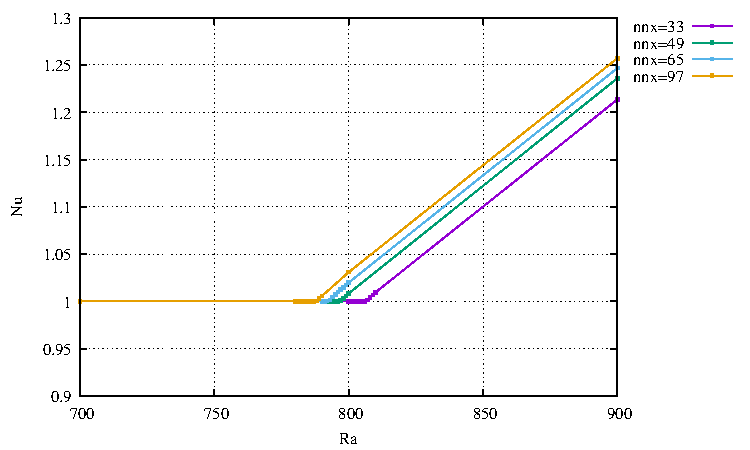
\includegraphics[width=8cm]{python_codes/fieldstone_155/results_onset/Ra_Nu.pdf}
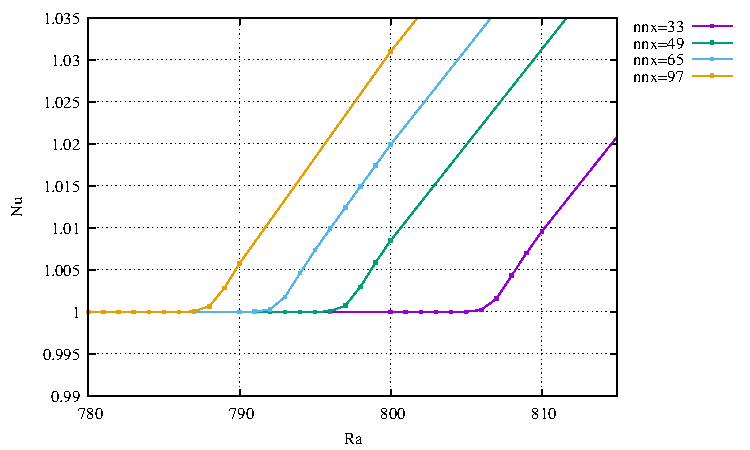
\includegraphics[width=8cm]{python_codes/fieldstone_155/results_onset/Ra_Nu_zoom.pdf}
\end{center}


\newpage
%%%%%%%%%%%%%%%%%%%%%%%%%%%%%%%%%%%%%%%%%%
\section*{Results: $\Ranb=10^{3,4,5,6}$, Steady state approach}

Results are obtained with {\tt script\_ss}. 

\begin{center}
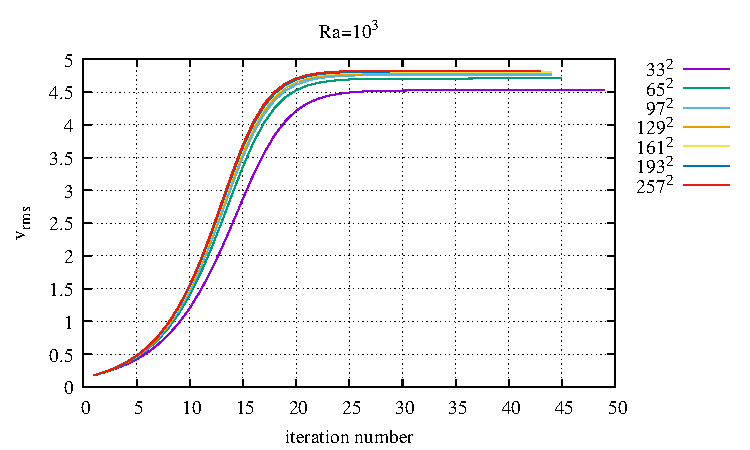
\includegraphics[width=4.297cm]{python_codes/fieldstone_155/results_SS/vrms_Ra1e3}
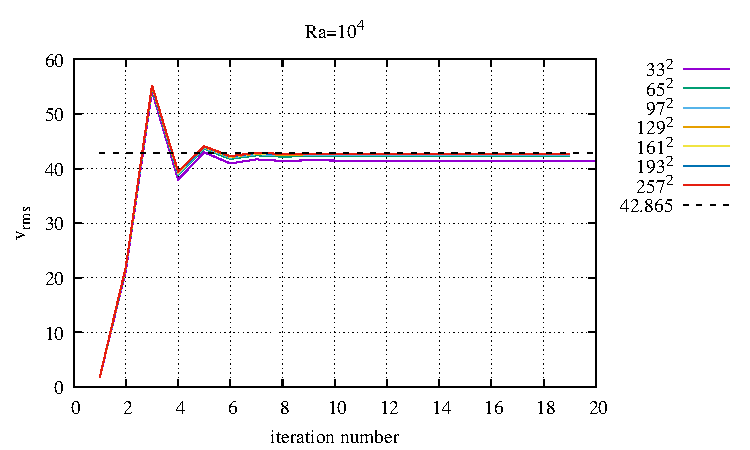
\includegraphics[width=4.297cm]{python_codes/fieldstone_155/results_SS/vrms_Ra1e4}
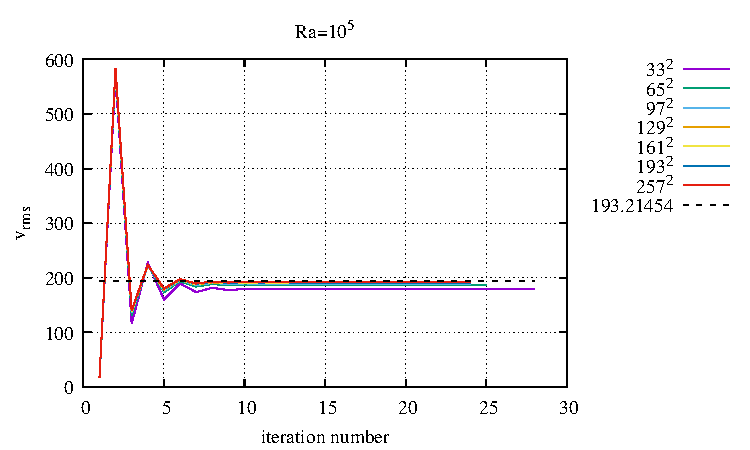
\includegraphics[width=4.297cm]{python_codes/fieldstone_155/results_SS/vrms_Ra1e5}
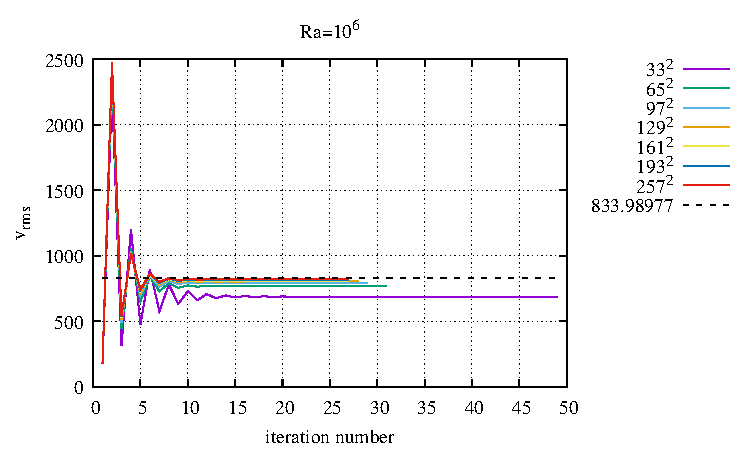
\includegraphics[width=4.297cm]{python_codes/fieldstone_155/results_SS/vrms_Ra1e6}\\
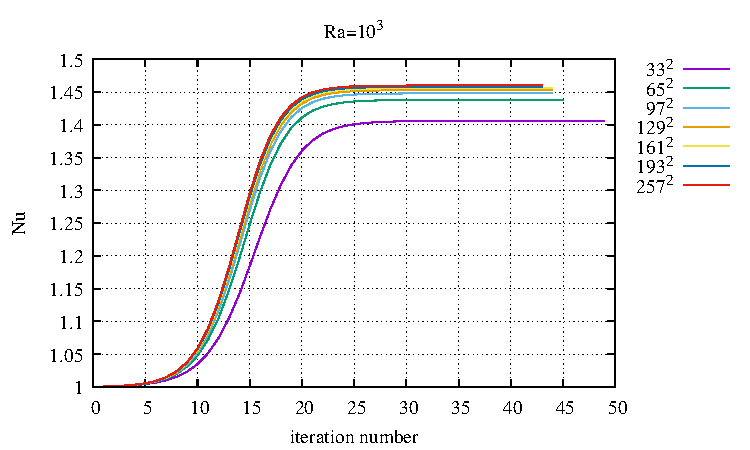
\includegraphics[width=4.297cm]{python_codes/fieldstone_155/results_SS/Nu_Ra1e3}
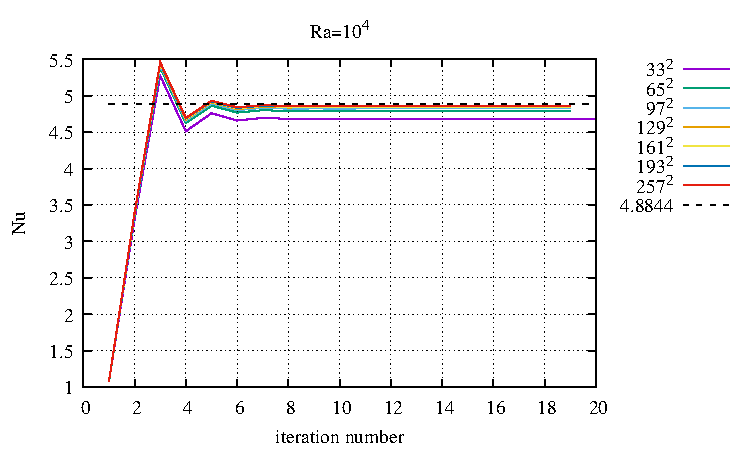
\includegraphics[width=4.297cm]{python_codes/fieldstone_155/results_SS/Nu_Ra1e4}
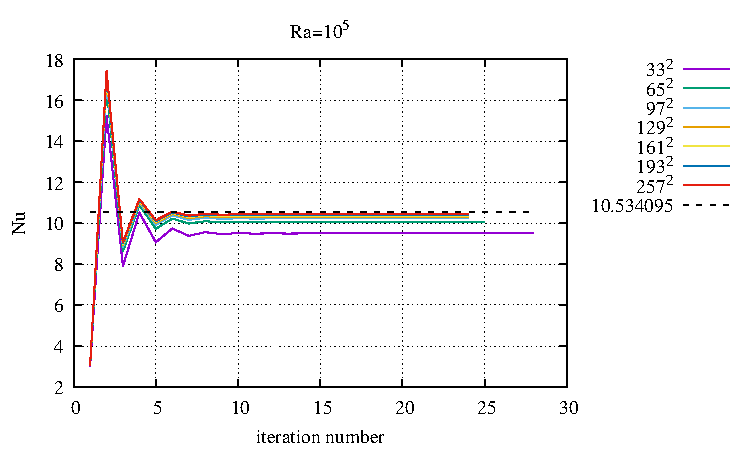
\includegraphics[width=4.297cm]{python_codes/fieldstone_155/results_SS/Nu_Ra1e5}
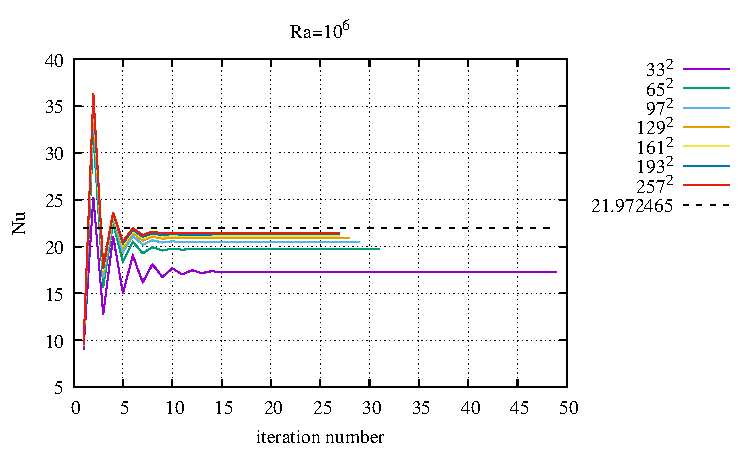
\includegraphics[width=4.297cm]{python_codes/fieldstone_155/results_SS/Nu_Ra1e6}
\end{center}

\begin{center}
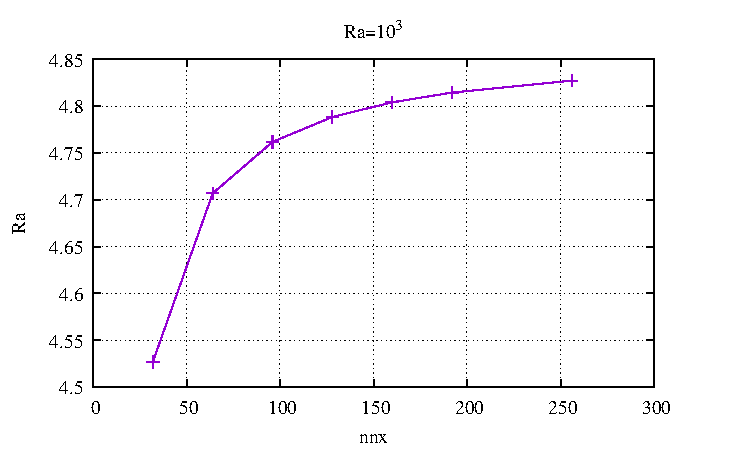
\includegraphics[width=4.297cm]{python_codes/fieldstone_155/results_SS/vrms1000}
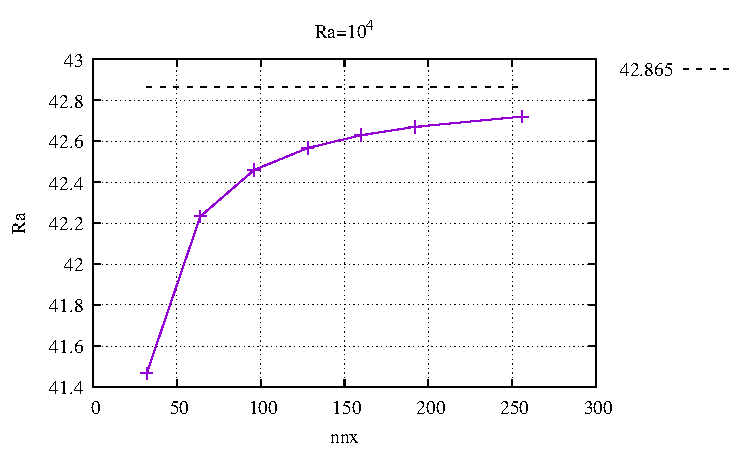
\includegraphics[width=4.297cm]{python_codes/fieldstone_155/results_SS/vrms10000}
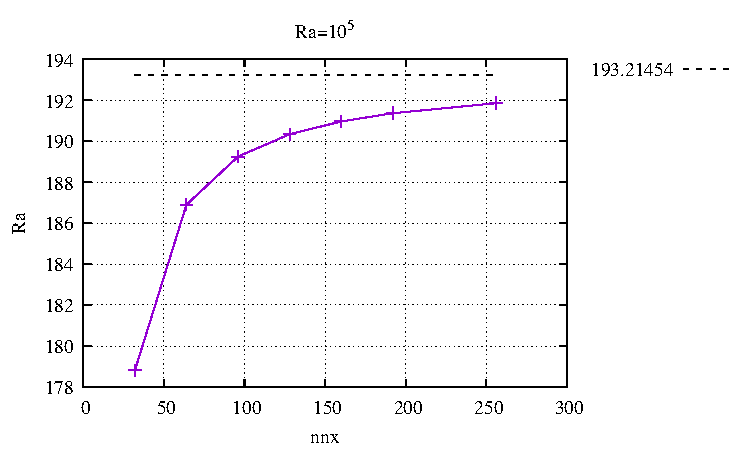
\includegraphics[width=4.297cm]{python_codes/fieldstone_155/results_SS/vrms100000}
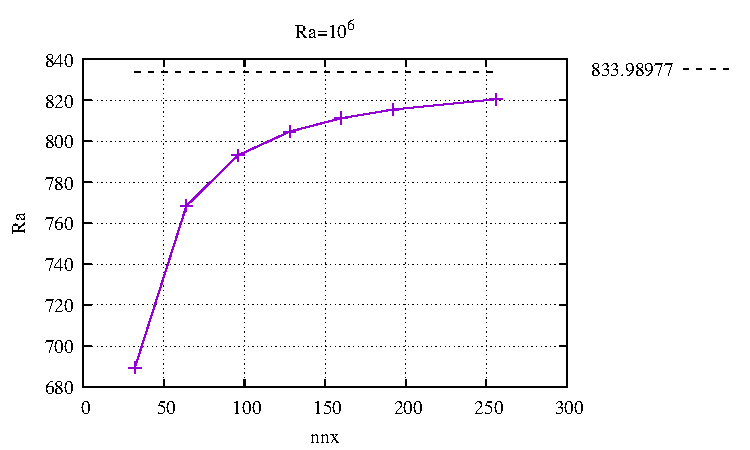
\includegraphics[width=4.297cm]{python_codes/fieldstone_155/results_SS/vrms1000000}\\
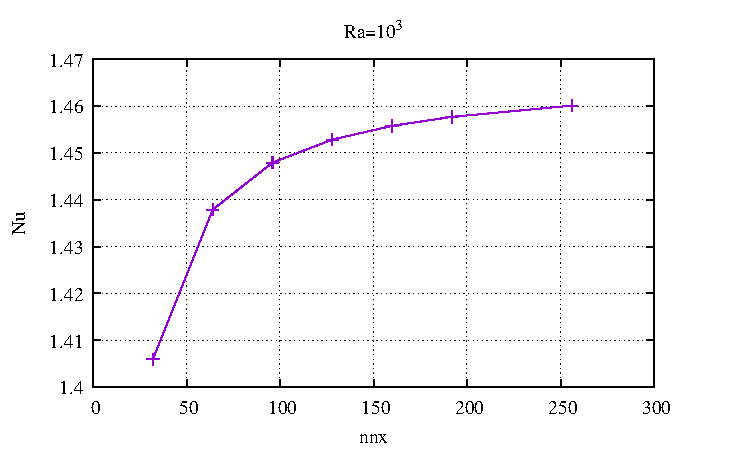
\includegraphics[width=4.297cm]{python_codes/fieldstone_155/results_SS/Nu1000}
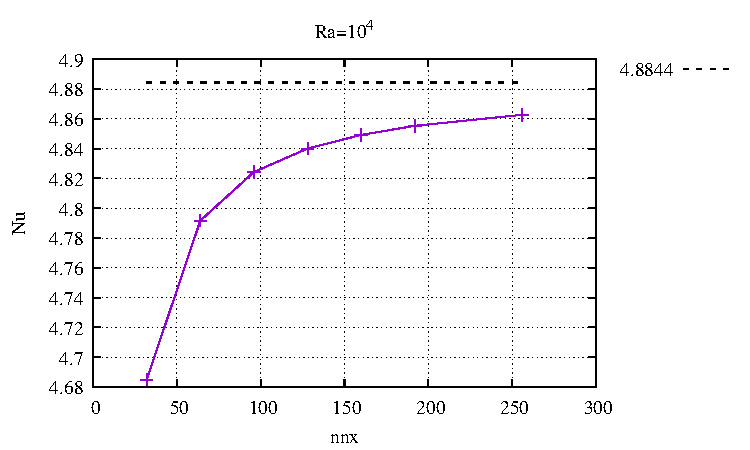
\includegraphics[width=4.297cm]{python_codes/fieldstone_155/results_SS/Nu10000}
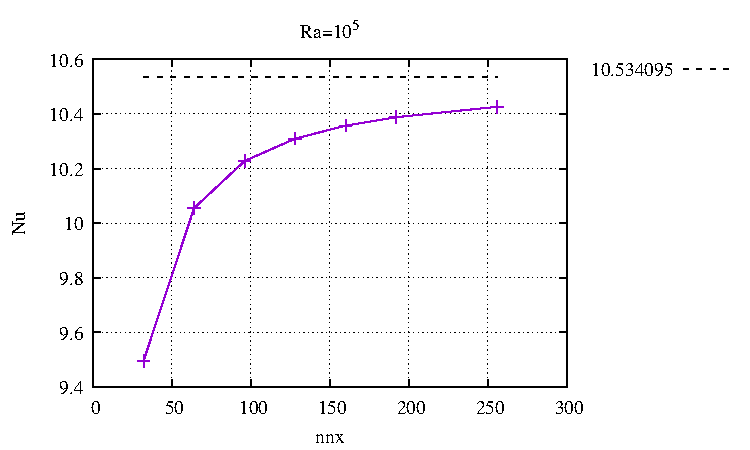
\includegraphics[width=4.297cm]{python_codes/fieldstone_155/results_SS/Nu100000}
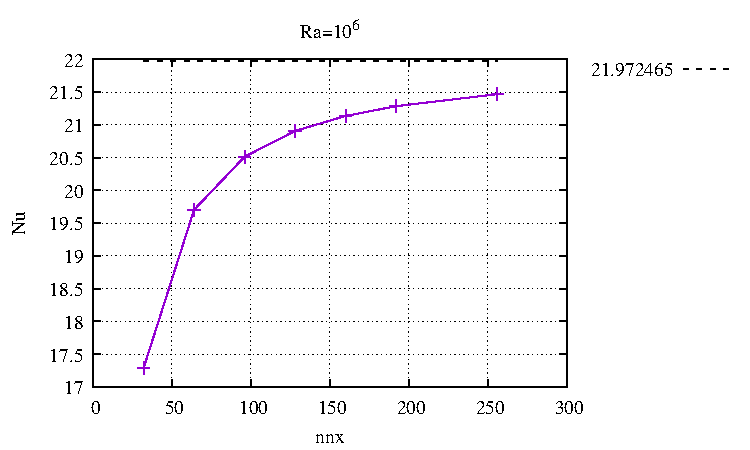
\includegraphics[width=4.297cm]{python_codes/fieldstone_155/results_SS/Nu1000000}
\end{center}



\newpage
%%%%%%%%%%%%%%%%%%%%%%%%%%%%%%%%%%%%%%%%%%
\section*{Results: $\Ranb=10^{3,4,5,6}$, CFL=0.5, time evolution}

\begin{center}
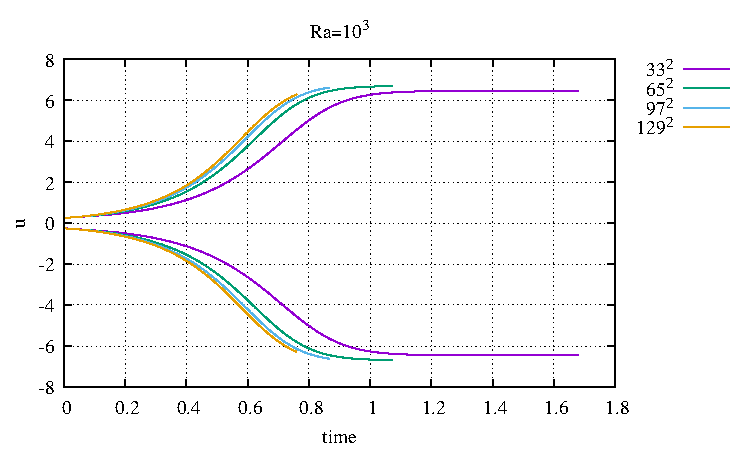
\includegraphics[width=4.297cm]{python_codes/fieldstone_155/results/stats_u_Ra1e3}
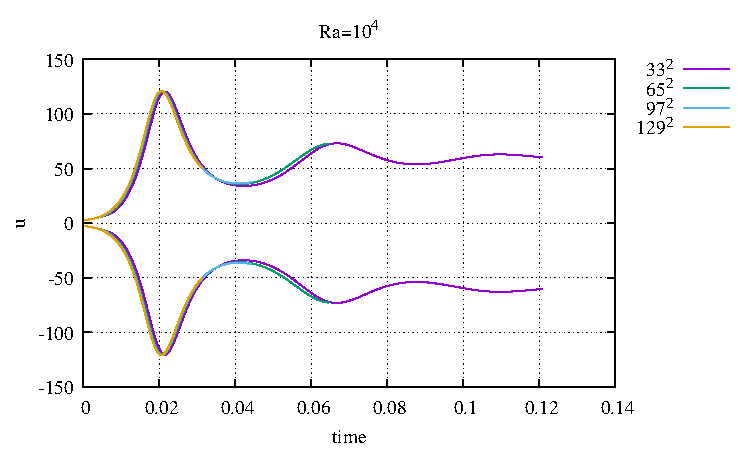
\includegraphics[width=4.297cm]{python_codes/fieldstone_155/results/stats_u_Ra1e4}
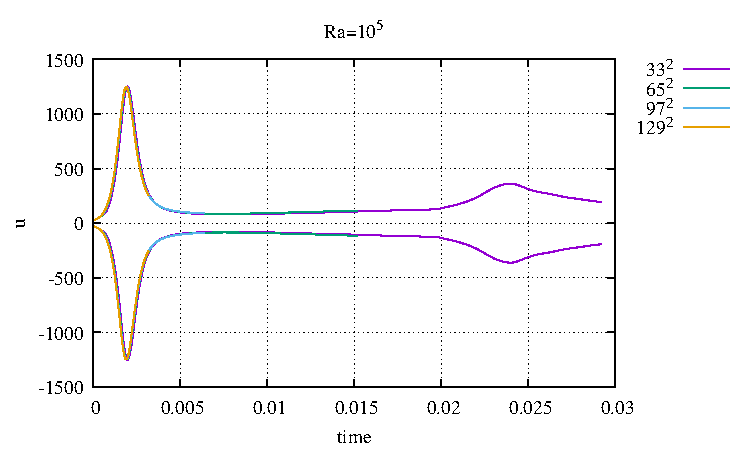
\includegraphics[width=4.297cm]{python_codes/fieldstone_155/results/stats_u_Ra1e5}
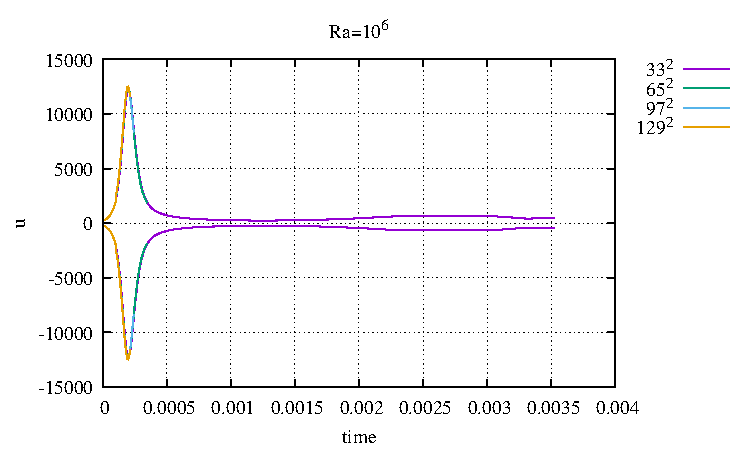
\includegraphics[width=4.297cm]{python_codes/fieldstone_155/results/stats_u_Ra1e6}\\
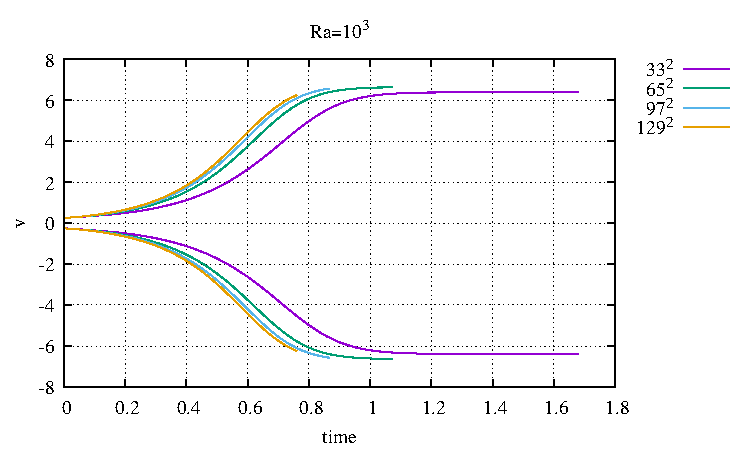
\includegraphics[width=4.297cm]{python_codes/fieldstone_155/results/stats_v_Ra1e3}
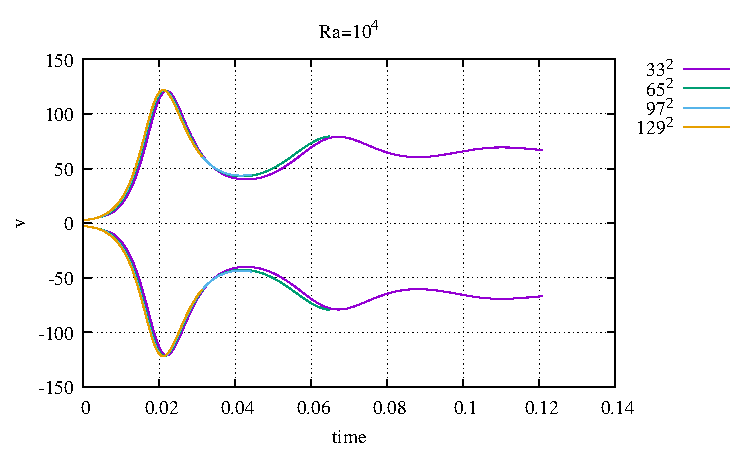
\includegraphics[width=4.297cm]{python_codes/fieldstone_155/results/stats_v_Ra1e4}
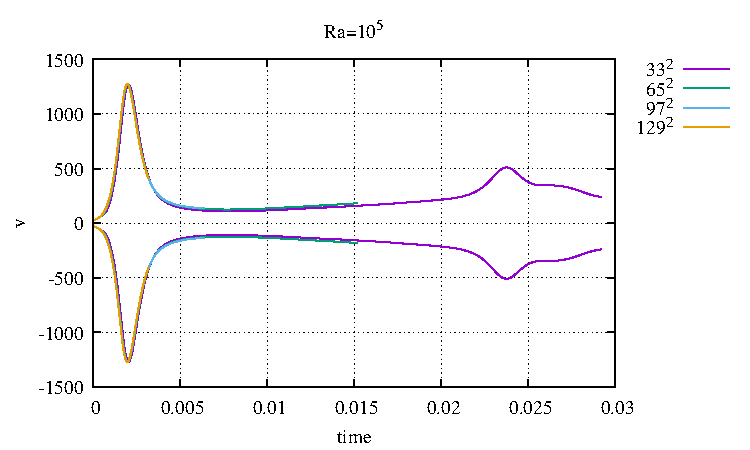
\includegraphics[width=4.297cm]{python_codes/fieldstone_155/results/stats_v_Ra1e5}
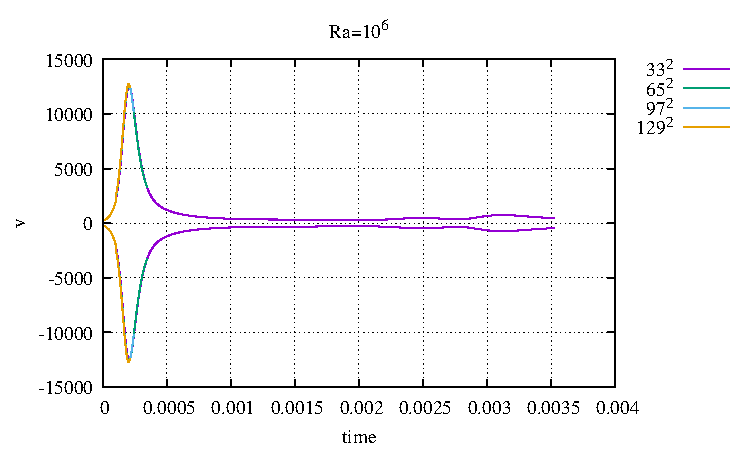
\includegraphics[width=4.297cm]{python_codes/fieldstone_155/results/stats_v_Ra1e6}\\
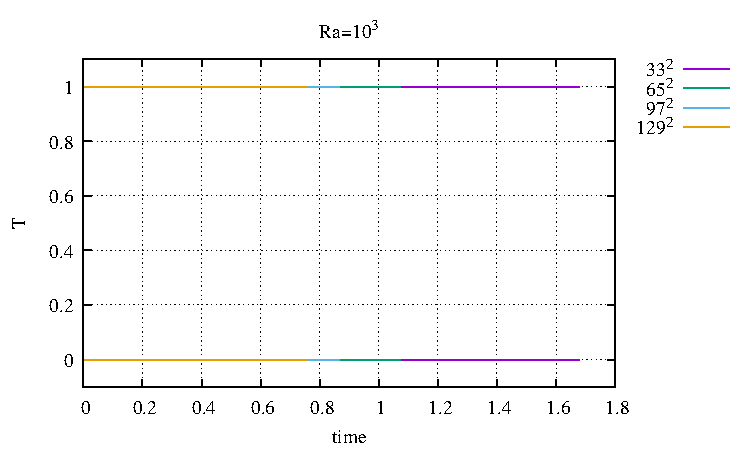
\includegraphics[width=4.297cm]{python_codes/fieldstone_155/results/stats_T_Ra1e3}
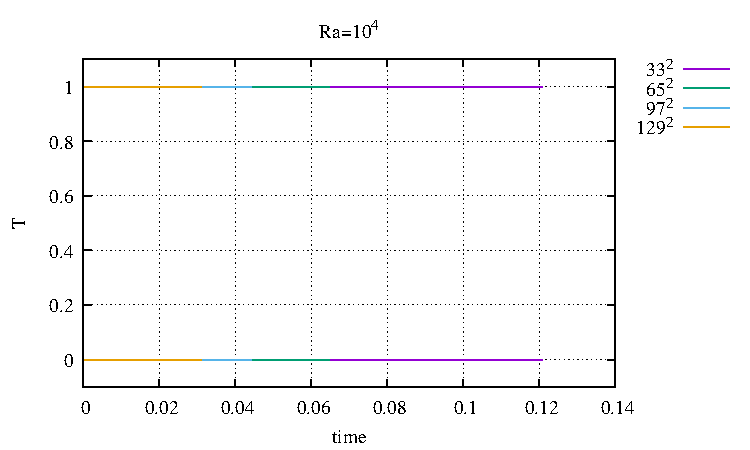
\includegraphics[width=4.297cm]{python_codes/fieldstone_155/results/stats_T_Ra1e4}
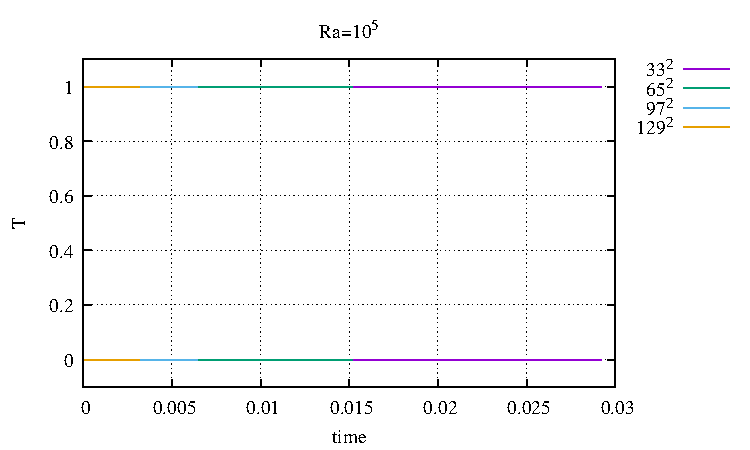
\includegraphics[width=4.297cm]{python_codes/fieldstone_155/results/stats_T_Ra1e5}
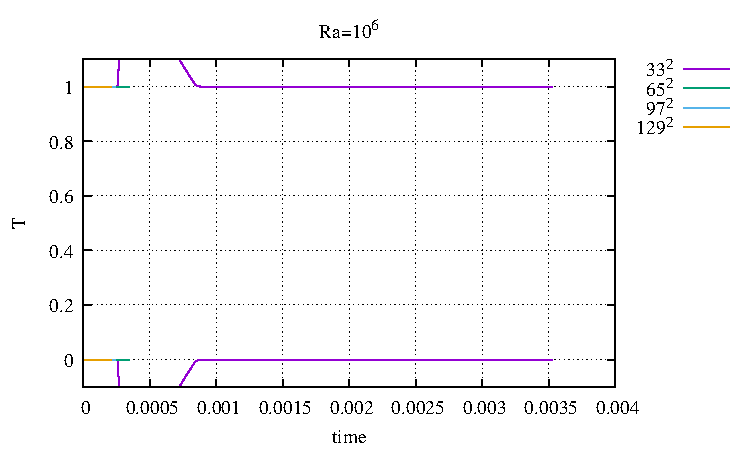
\includegraphics[width=4.297cm]{python_codes/fieldstone_155/results/stats_T_Ra1e6}\\
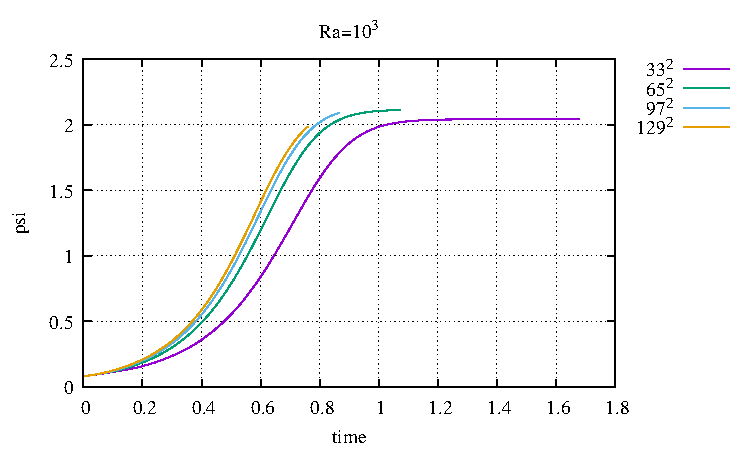
\includegraphics[width=4.297cm]{python_codes/fieldstone_155/results/stats_psi_Ra1e3}
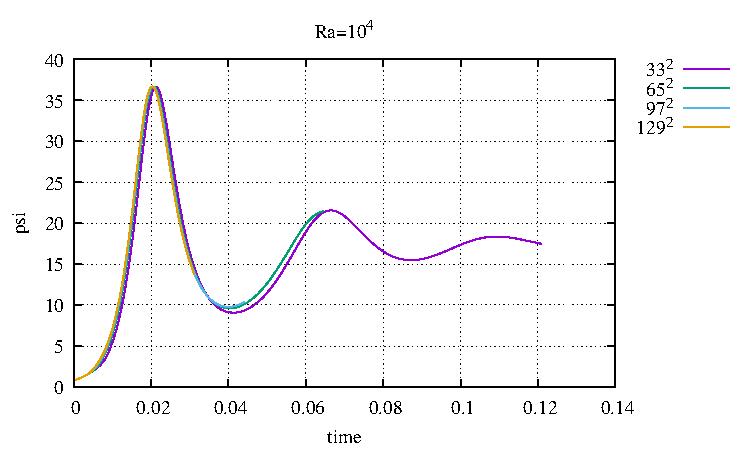
\includegraphics[width=4.297cm]{python_codes/fieldstone_155/results/stats_psi_Ra1e4}
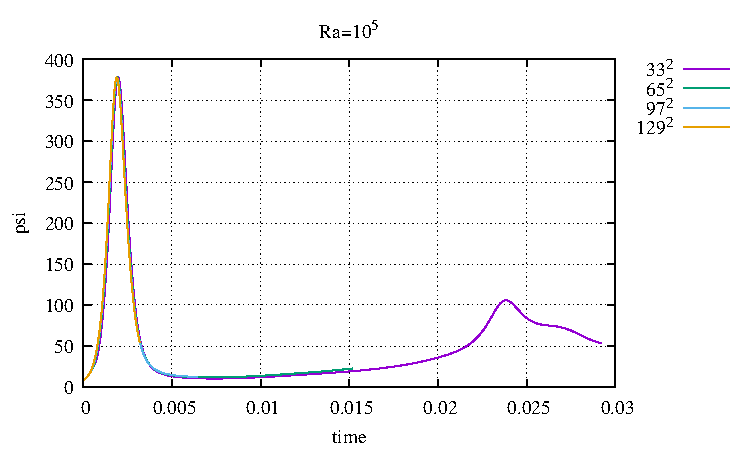
\includegraphics[width=4.297cm]{python_codes/fieldstone_155/results/stats_psi_Ra1e5}
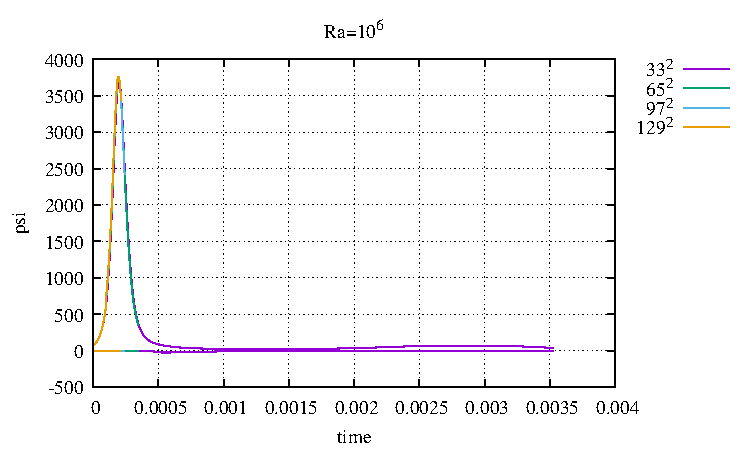
\includegraphics[width=4.297cm]{python_codes/fieldstone_155/results/stats_psi_Ra1e6}\\
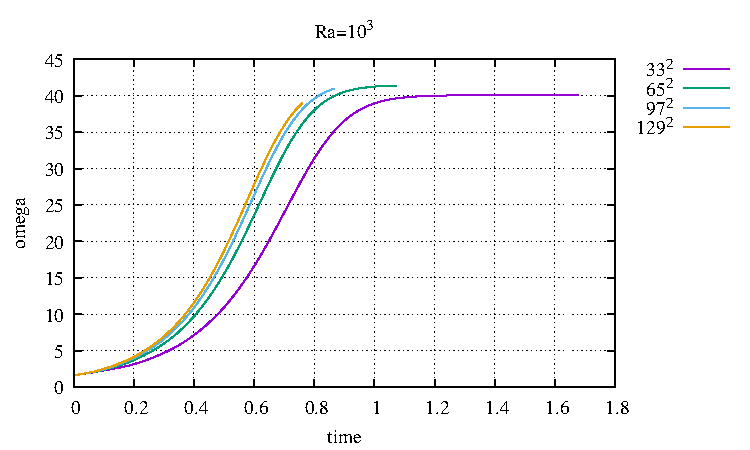
\includegraphics[width=4.297cm]{python_codes/fieldstone_155/results/stats_omega_Ra1e3}
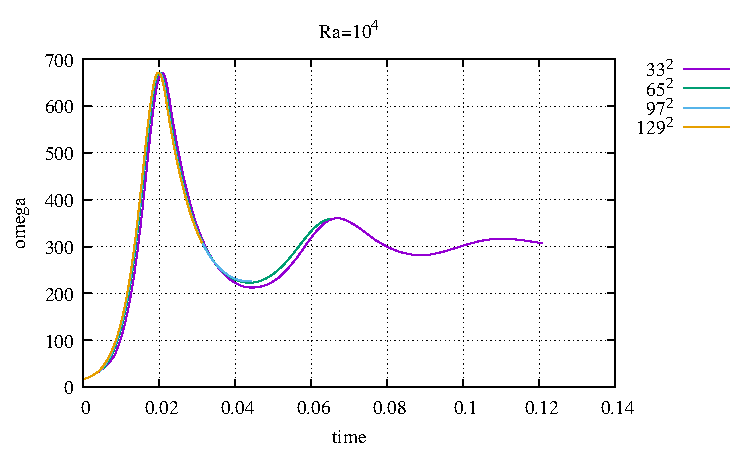
\includegraphics[width=4.297cm]{python_codes/fieldstone_155/results/stats_omega_Ra1e4}
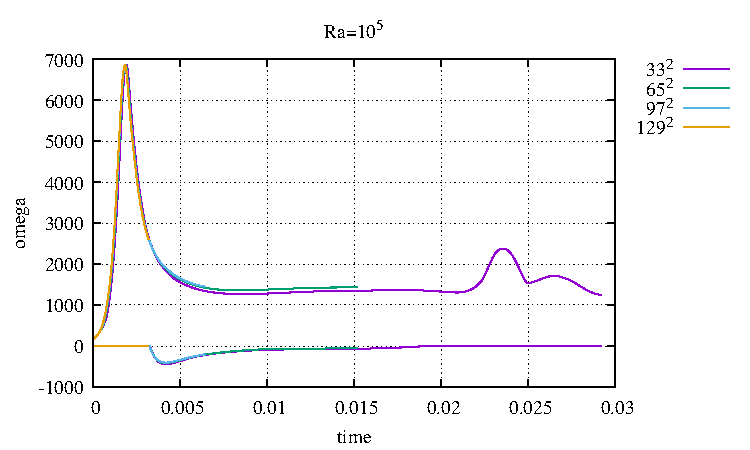
\includegraphics[width=4.297cm]{python_codes/fieldstone_155/results/stats_omega_Ra1e5}
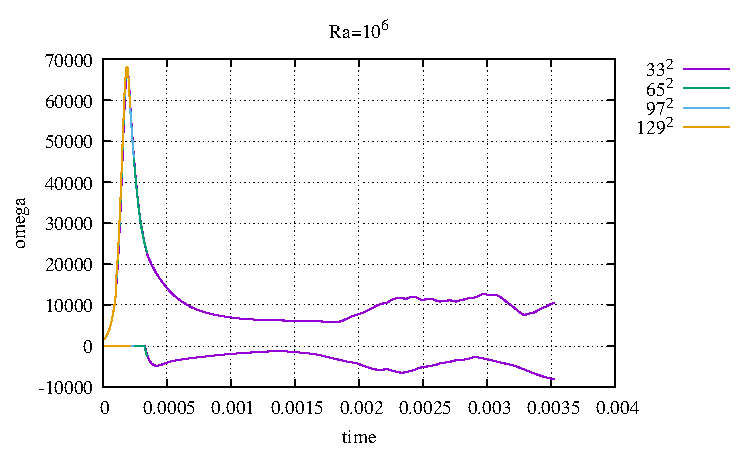
\includegraphics[width=4.297cm]{python_codes/fieldstone_155/results/stats_omega_Ra1e6}
\\
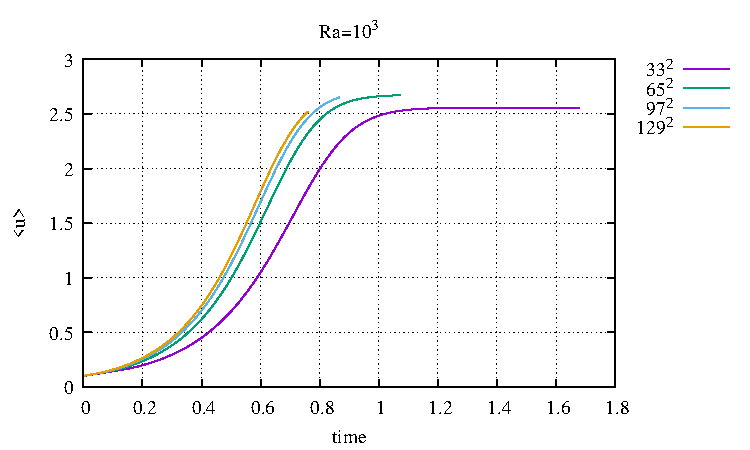
\includegraphics[width=4.297cm]{python_codes/fieldstone_155/results/avrg_u_Ra1e3}
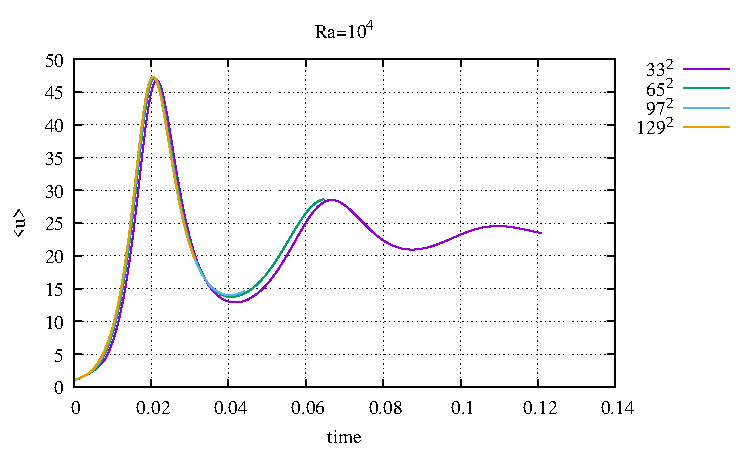
\includegraphics[width=4.297cm]{python_codes/fieldstone_155/results/avrg_u_Ra1e4}
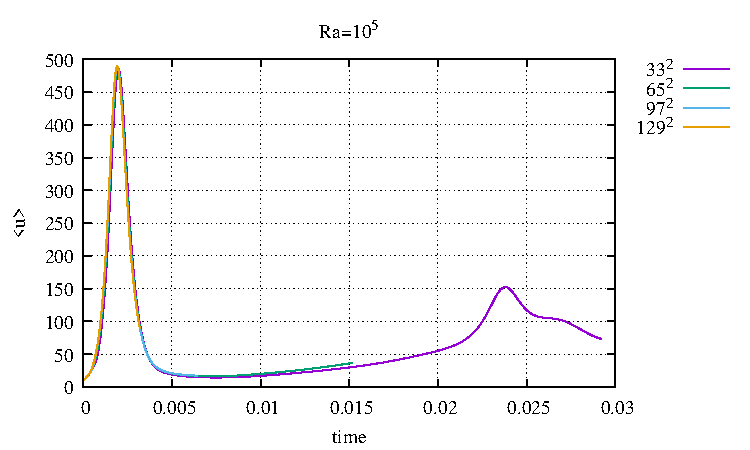
\includegraphics[width=4.297cm]{python_codes/fieldstone_155/results/avrg_u_Ra1e5}
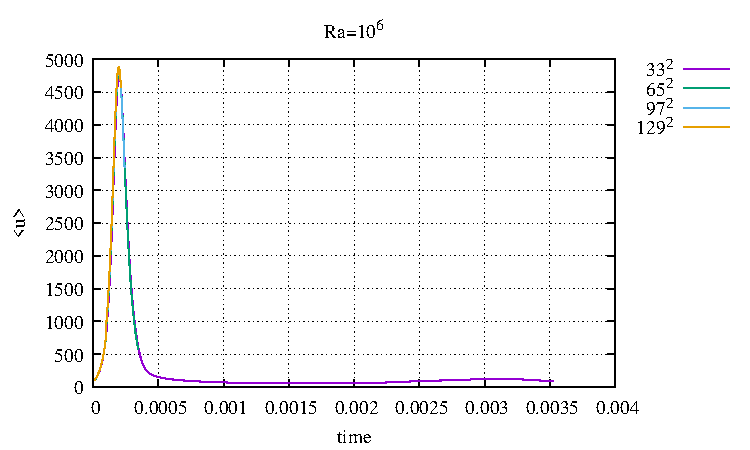
\includegraphics[width=4.297cm]{python_codes/fieldstone_155/results/avrg_u_Ra1e6}\\
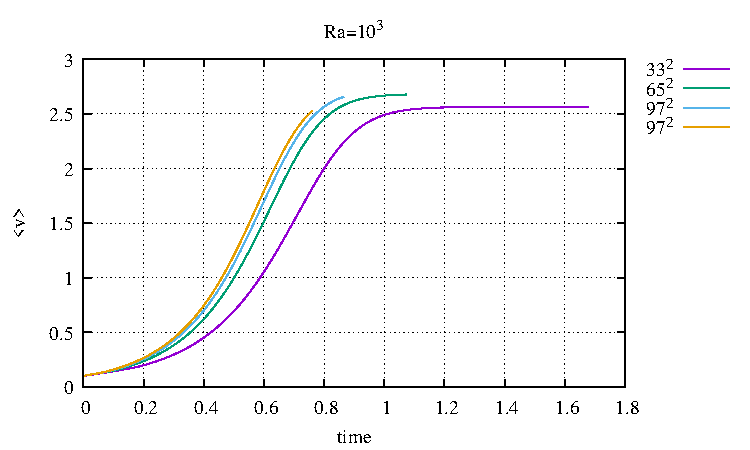
\includegraphics[width=4.297cm]{python_codes/fieldstone_155/results/avrg_v_Ra1e3}
\includegraphics[width=4.297cm]{python_codes/fieldstone_155/results/avrg_v_Ra1e4}
\includegraphics[width=4.297cm]{python_codes/fieldstone_155/results/avrg_v_Ra1e5}
\includegraphics[width=4.297cm]{python_codes/fieldstone_155/results/avrg_v_Ra1e6}\\
\includegraphics[width=4.297cm]{python_codes/fieldstone_155/results/avrg_T_Ra1e3}
\includegraphics[width=4.297cm]{python_codes/fieldstone_155/results/avrg_T_Ra1e4}
\includegraphics[width=4.297cm]{python_codes/fieldstone_155/results/avrg_T_Ra1e5}
\includegraphics[width=4.297cm]{python_codes/fieldstone_155/results/avrg_T_Ra1e6}
\\
\includegraphics[width=4.297cm]{python_codes/fieldstone_155/results/vrms_Ra1e3}
\includegraphics[width=4.297cm]{python_codes/fieldstone_155/results/vrms_Ra1e4}
\includegraphics[width=4.297cm]{python_codes/fieldstone_155/results/vrms_Ra1e5}
\includegraphics[width=4.297cm]{python_codes/fieldstone_155/results/vrms_Ra1e6}\\
\includegraphics[width=4.297cm]{python_codes/fieldstone_155/results/Nu_Ra1e3}
\includegraphics[width=4.297cm]{python_codes/fieldstone_155/results/Nu_Ra1e4}
\includegraphics[width=4.297cm]{python_codes/fieldstone_155/results/Nu_Ra1e5}
\includegraphics[width=4.297cm]{python_codes/fieldstone_155/results/Nu_Ra1e6}
\\
\includegraphics[width=4.297cm]{python_codes/fieldstone_155/results/conv_u_Ra1e3}
\includegraphics[width=4.297cm]{python_codes/fieldstone_155/results/conv_u_Ra1e4}
\includegraphics[width=4.297cm]{python_codes/fieldstone_155/results/conv_u_Ra1e5}
\includegraphics[width=4.297cm]{python_codes/fieldstone_155/results/conv_u_Ra1e6}\\
\includegraphics[width=4.297cm]{python_codes/fieldstone_155/results/conv_v_Ra1e3}
\includegraphics[width=4.297cm]{python_codes/fieldstone_155/results/conv_v_Ra1e4}
\includegraphics[width=4.297cm]{python_codes/fieldstone_155/results/conv_v_Ra1e5}
\includegraphics[width=4.297cm]{python_codes/fieldstone_155/results/conv_v_Ra1e6}\\
\includegraphics[width=4.297cm]{python_codes/fieldstone_155/results/conv_T_Ra1e3}
\includegraphics[width=4.297cm]{python_codes/fieldstone_155/results/conv_T_Ra1e4}
\includegraphics[width=4.297cm]{python_codes/fieldstone_155/results/conv_T_Ra1e5}
\includegraphics[width=4.297cm]{python_codes/fieldstone_155/results/conv_T_Ra1e6}\\
\includegraphics[width=4.297cm]{python_codes/fieldstone_155/results/conv_psi_Ra1e3}
\includegraphics[width=4.297cm]{python_codes/fieldstone_155/results/conv_psi_Ra1e4}
\includegraphics[width=4.297cm]{python_codes/fieldstone_155/results/conv_psi_Ra1e5}
\includegraphics[width=4.297cm]{python_codes/fieldstone_155/results/conv_psi_Ra1e6}\\
\includegraphics[width=4.297cm]{python_codes/fieldstone_155/results/conv_omega_Ra1e3}
\includegraphics[width=4.297cm]{python_codes/fieldstone_155/results/conv_omega_Ra1e4}
\includegraphics[width=4.297cm]{python_codes/fieldstone_155/results/conv_omega_Ra1e5}
\includegraphics[width=4.297cm]{python_codes/fieldstone_155/results/conv_omega_Ra1e6}\\
\end{center}

%%%%%%%%%%%%%%%%%%%%%%%%%%%%%%%%%%%%%%%%%%%%%%%%%%%%%%%%%%%%%%%%%%%%%%%%%%%%%%%%%%%%%%%%%%%%%%%%%%%
\par\noindent\rule{\textwidth}{0.4pt}

\vspace{.5cm}

\begin{center}
\fbox{\begin{minipage}{0.9\textwidth}
{\color{teal}To Do, open questions, future work?}
\begin{itemize}
\item compute dTdx,dTdy with second order accurate stencil on boundary too
\item run all to steady state
\end{itemize}
\end{minipage}}
\end{center}


